\documentclass[aspectratio=169]{beamer}

% \usefonttheme{Serif}

\usepackage{physics}
\usepackage[export]{adjustbox}
\usepackage[absolute,overlay]{textpos}
\usepackage{graphicx}

\usepackage{derivative}
% I should not have to do this
\DeclareOdvVariant{\odv}{d}[style-inf=\mathrm] 


% \title{Kiral perturbasjonsteori}

\author{Martin Johnsrud}

\begin{document}
    % \frame{\titlepage}

    \begin{frame}
        \frametitle{Pion stars}
        \begin{itemize}
            \item New proposal: stars made of pions
            \item Microscopic part: what are the\\ thermodynamics of pions?
            \item Macroscopic part: hydrodynamics of\\
             astrophysical objects
            \item Questions: What are the mass-radius\\
            relations of pion stars?
            How do EM-interactions/including three quarks/loop corrections influence the star?
        \end{itemize}

        \begin{textblock}{8}(8, 1)
            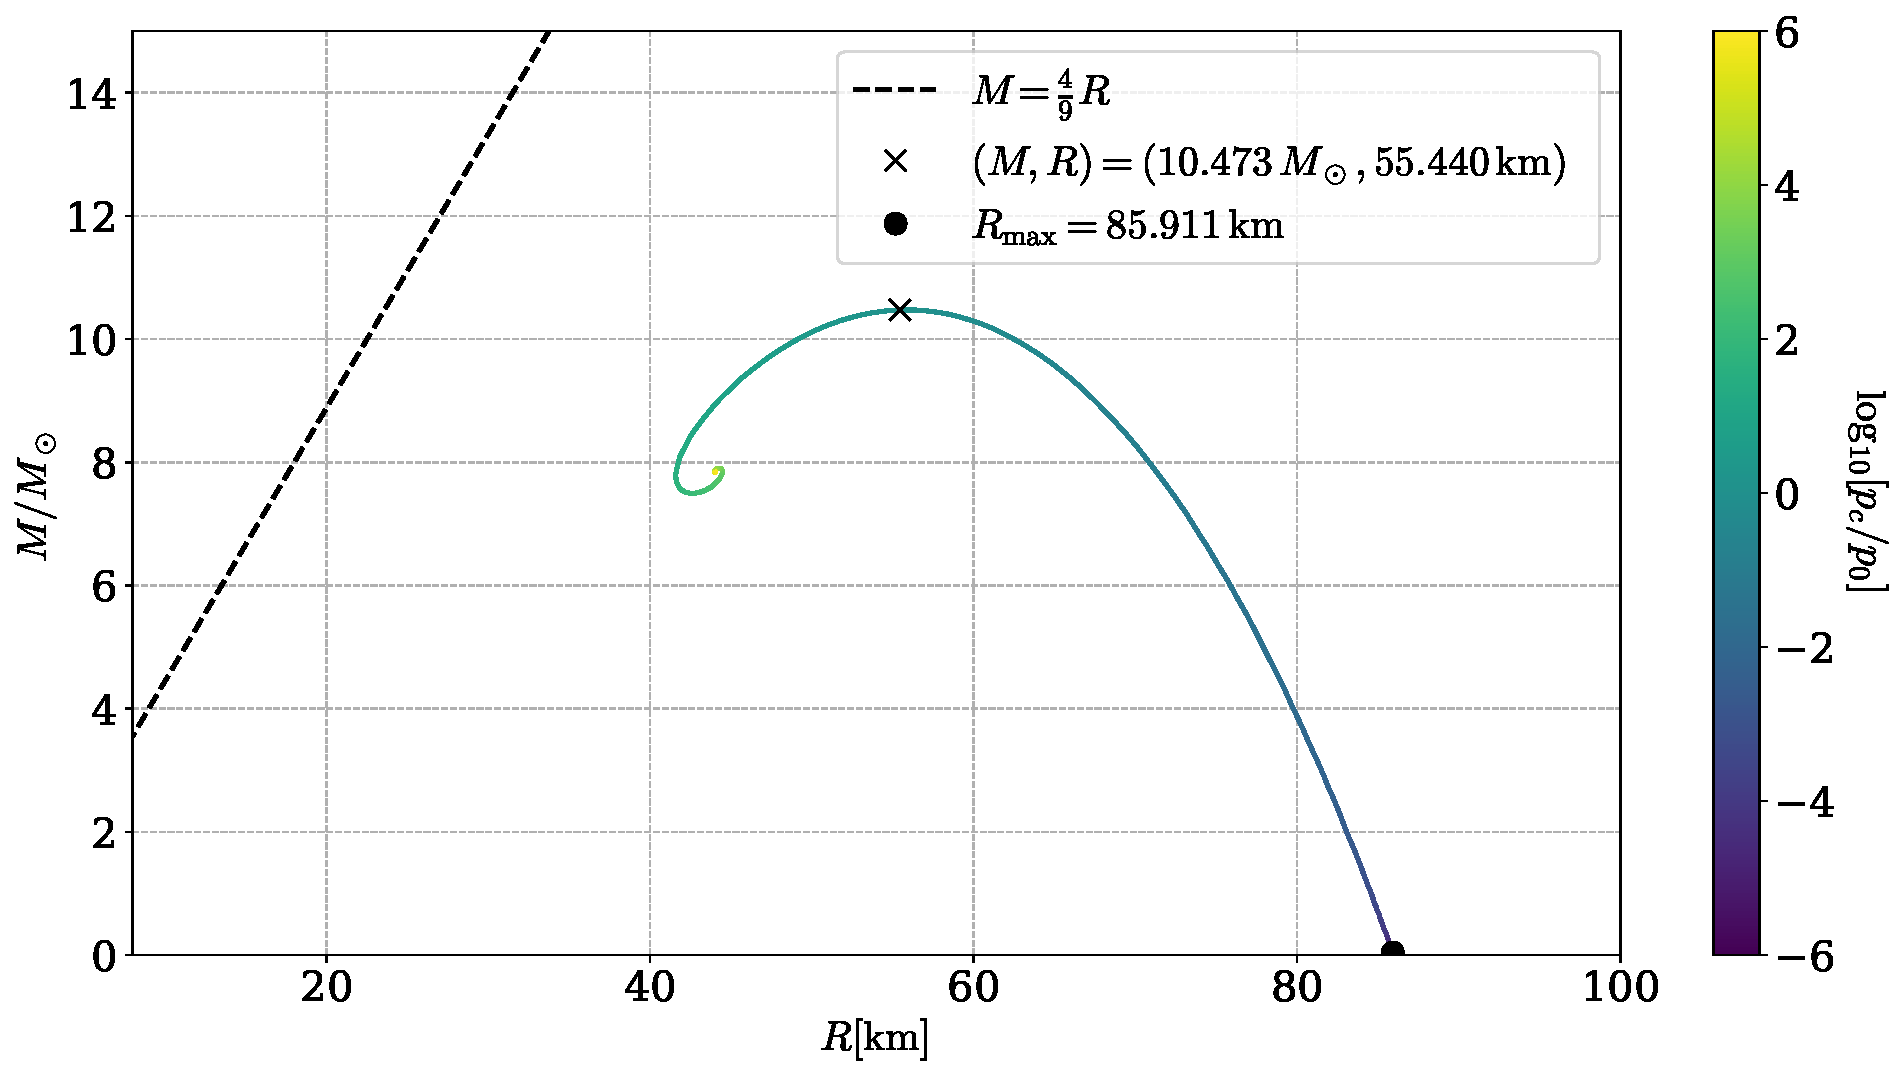
\includegraphics[width=\textwidth]{../../scripts/figurer/pion_star/mass_radius_pion_star.pdf}
        \end{textblock}


    \end{frame}

    \begin{frame}

        \frametitle{Thermodynamics of quarks}

        \begin{textblock}{4.8}(10.5, 1)
            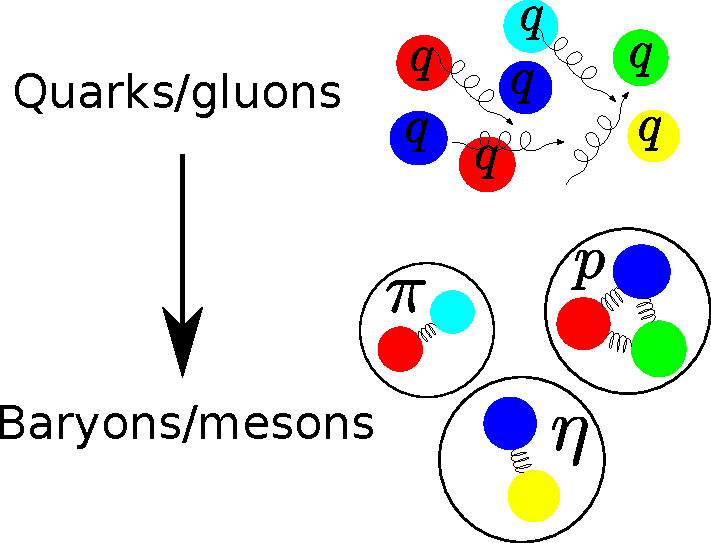
\includegraphics[width=\textwidth]{quarks-to-mesons.pdf}
        \end{textblock}
        \begin{textblock}{6}(9, 8)
            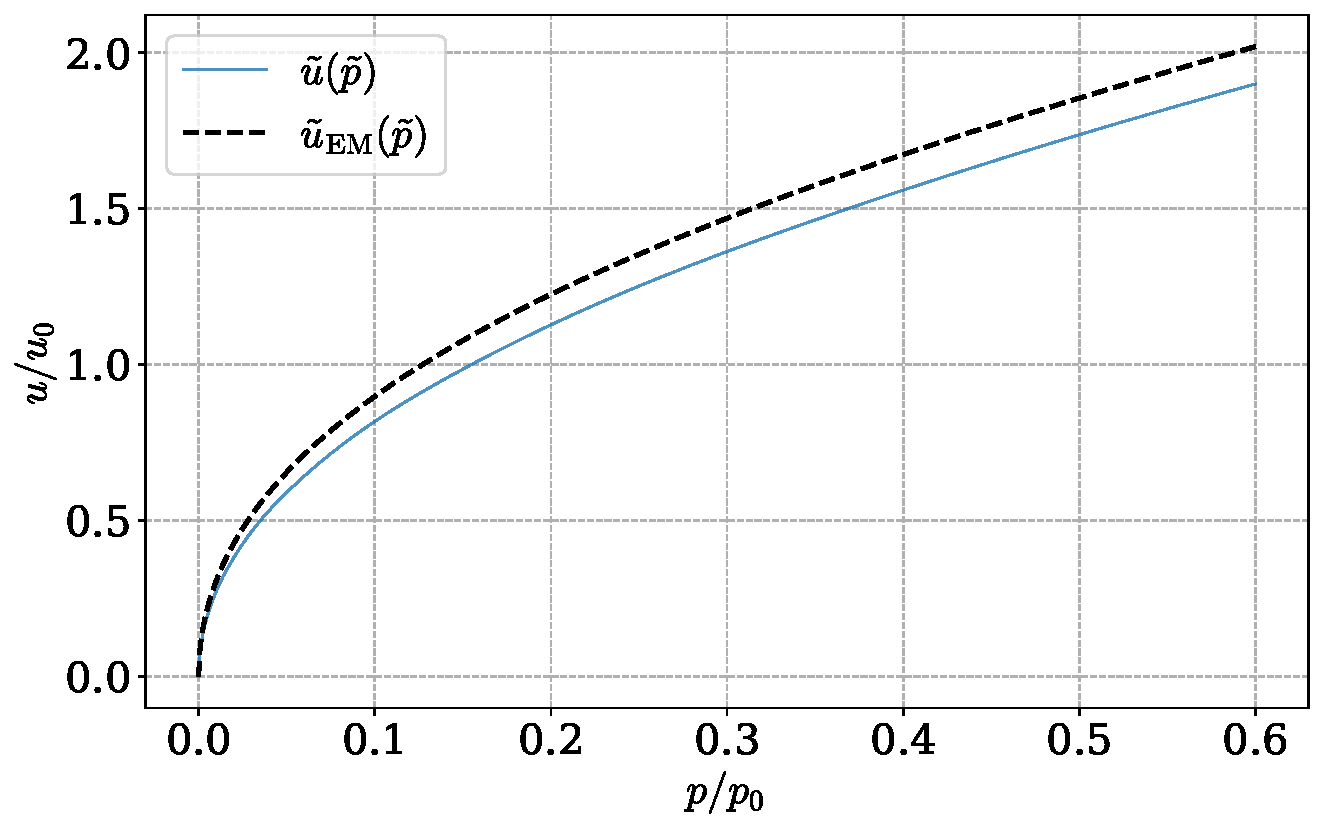
\includegraphics[width=\textwidth]{../../scripts/figurer/pion_star/pion_eos_EM.pdf}
        \end{textblock}


        \begin{itemize}
            \itemsep 0.4cm
            \item Effective theory for QCD: Chiral perturbation theory\\
            $
            \mathcal L = 
            \sum_f \bar q_f (\gamma^\mu [\partial_\mu - i q     \lambda^a A^a_\mu ] + m_f)q_f
            + G^a_{\mu \nu} G_a^{\mu \nu}
            $ \\
            $
            \longrightarrow
            \frac{1}{4} f^2 \Tr{\nabla_\mu \Sigma (\nabla^\mu \Sigma)^\dagger}
            + \frac{1}{4} f^2 \Tr{\chi^\dagger \Sigma + \Sigma^\dagger \chi} 
            $\\
            $
            \quad\quad + \frac{1}{3} l_1 \Tr{\nabla_\mu \Sigma (\nabla^\mu \Sigma)^\dagger}^2+
            ..., \quad
            \Sigma \in \text{SU}(3).
            $
            \item $\Sigma 
            = e^{i\alpha \lambda_2/2}\exp\left\{i \pi_a \lambda_a / f\right\}e^{i\alpha \lambda_2/2}
            $
            \item Free energy
            $
            F = - T
            \ln\Big[\int \mathcal{D}\pi e^{-S}\Big]
            $
            \item Include isospin and strangeness chemical \\
            potential, EM-interactions, loops...
            \item Phase transitions: pion condensation
            \item Calculate equation of state
        \end{itemize}


    \end{frame}

    \begin{frame}
        \frametitle{Hydrostatic equilibrium}

        \begin{columns}
        \begin{column}{0.4\textwidth}


        \begin{itemize}
            \item TOV equation govern pressure of perfect fluids in hydrostatic equilibrium\\
            $
            \odv{P}{r} = - \frac{G}{r^2} 
            \frac{\left(u + P\right)
            \left(m + 4 \pi r^3 P\right)}
            {\left(1 - \frac{2Gm}{r} \right)}
            ,
            $ \\
            $
            \odv{m}{r} = 4 \pi r^2 u
            $
            \item Numerical integration gives $P$, $u$ and thus $M$, $R$. 
        \end{itemize}

        \end{column}
        \begin{column}{0.6\textwidth}
            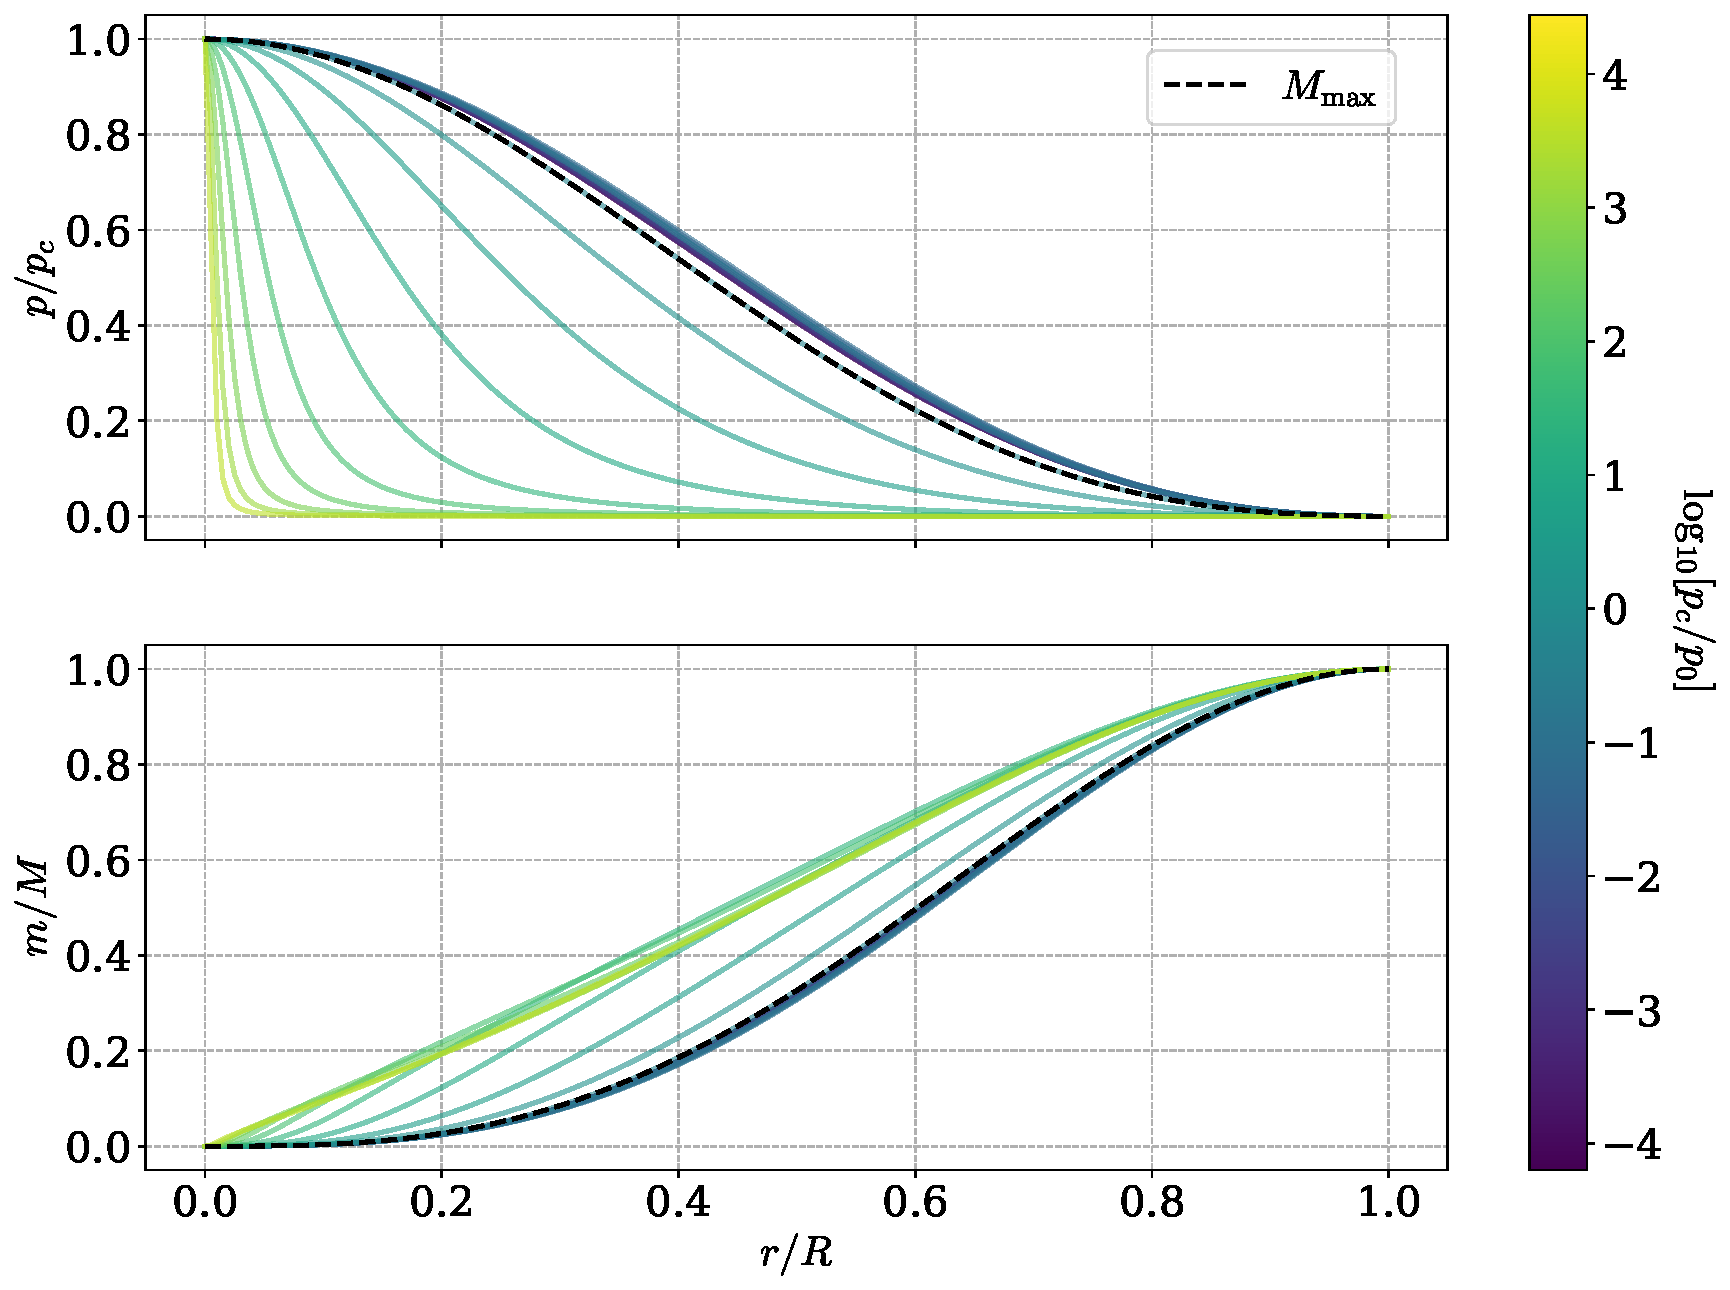
\includegraphics[width=\textwidth]{../../scripts/figurer/pion_star/pressure_mass_pion_star.pdf}
        \end{column}
        \end{columns}
    \end{frame}

    \begin{frame}
        \frametitle{Spot the difference}
        \begin{columns}
            \begin{column}{0.5\textwidth}
                Neutron star
                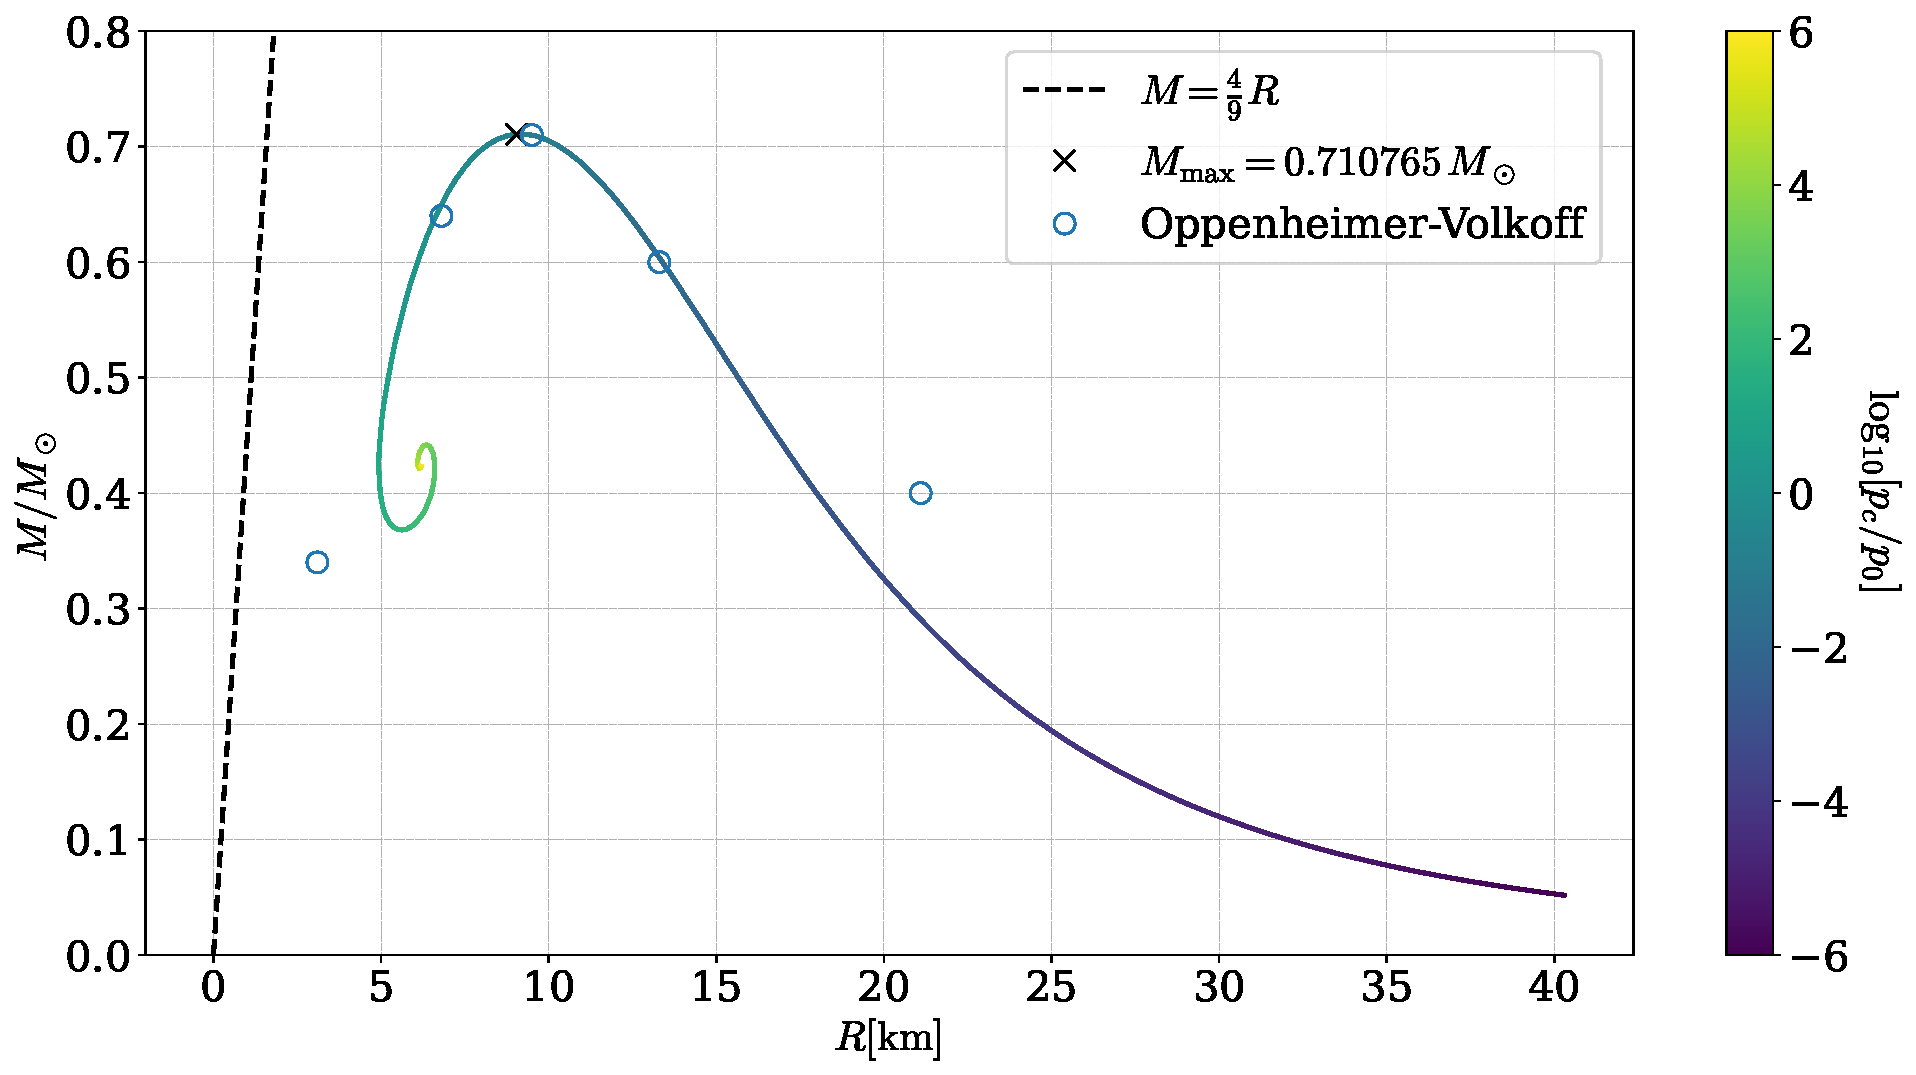
\includegraphics[width=\textwidth]{../../scripts/figurer/mass_radius_neutron.pdf}
            \end{column}
            \begin{column}{0.5\textwidth}
                Pion star
                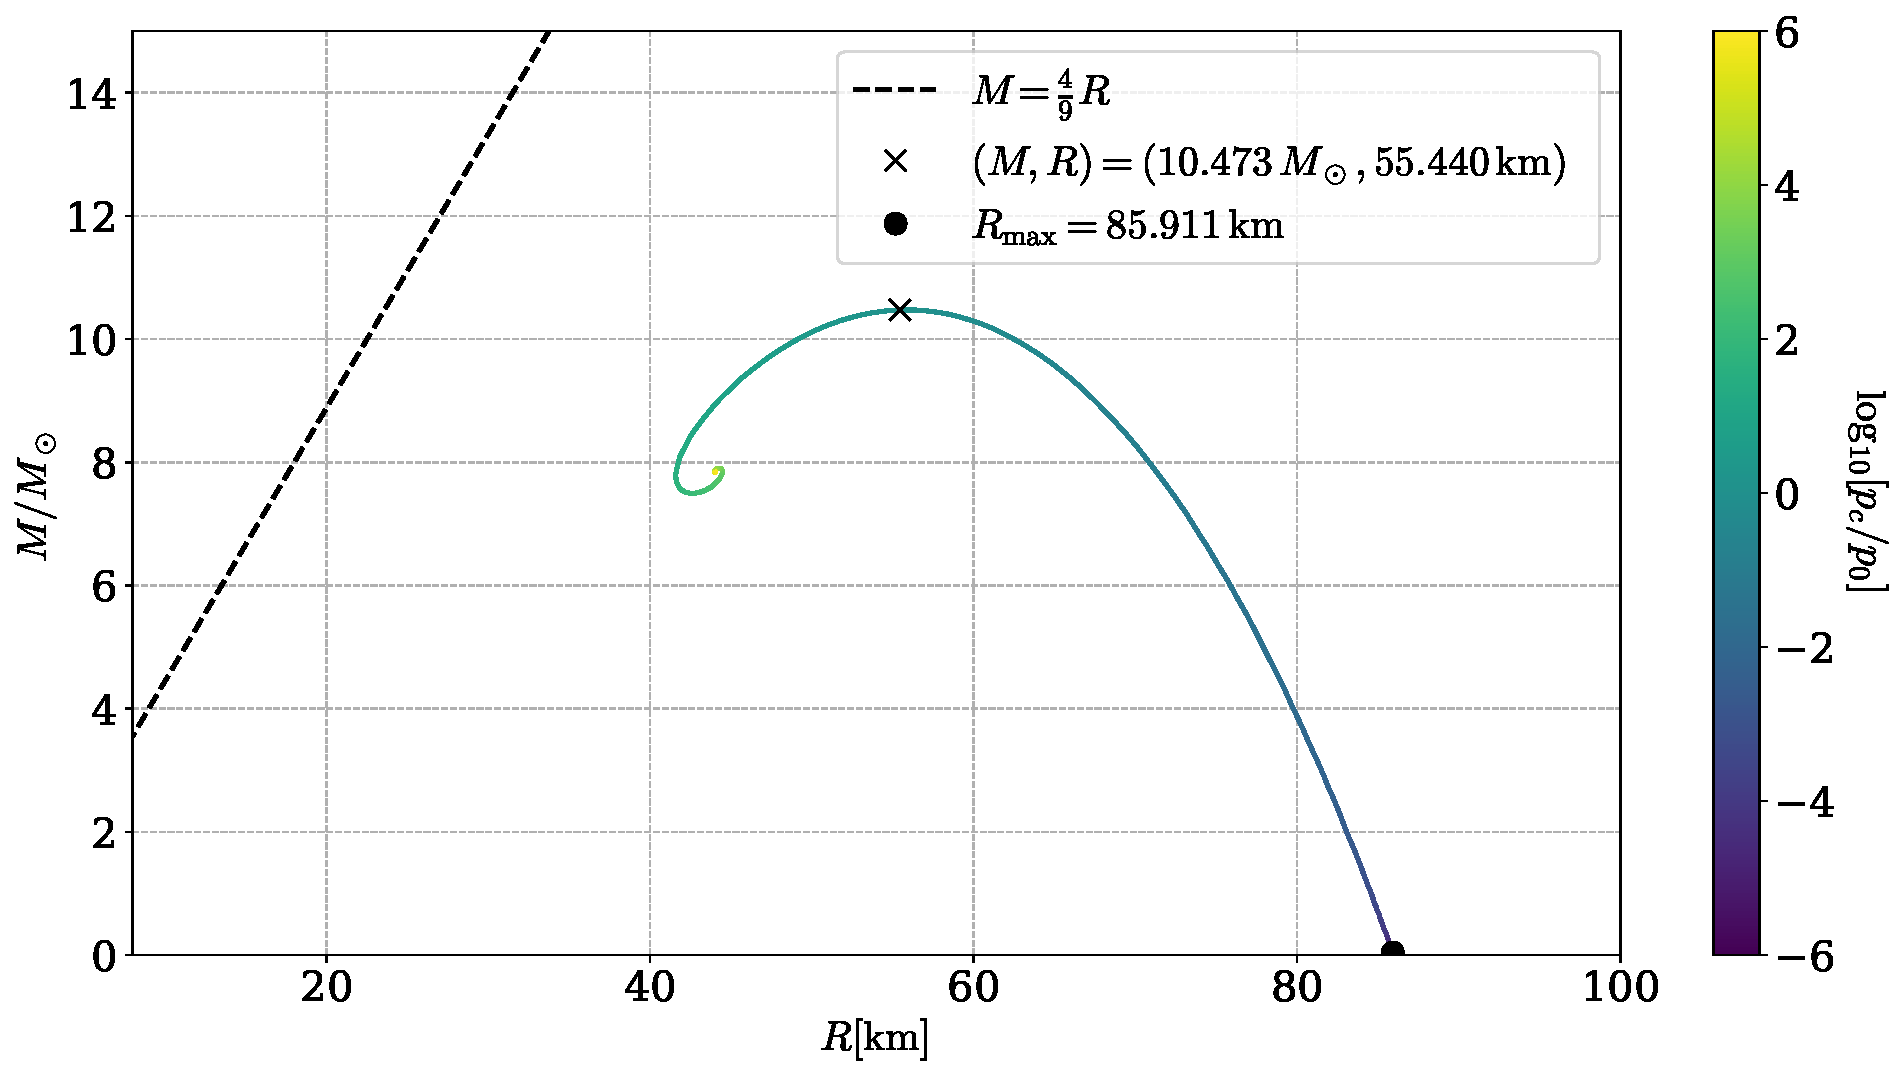
\includegraphics[width=\textwidth]{../../scripts/figurer/pion_star/mass_radius_pion_star.pdf}
            \end{column}
        \end{columns}
        Why does pion star have a maximum radius? As far as we can tell, no one has commented or given an explanation.
    \end{frame}

    \begin{frame}
        \frametitle{Non-relativistic approximation}

        \begin{textblock}{8}(8, 1.2)
            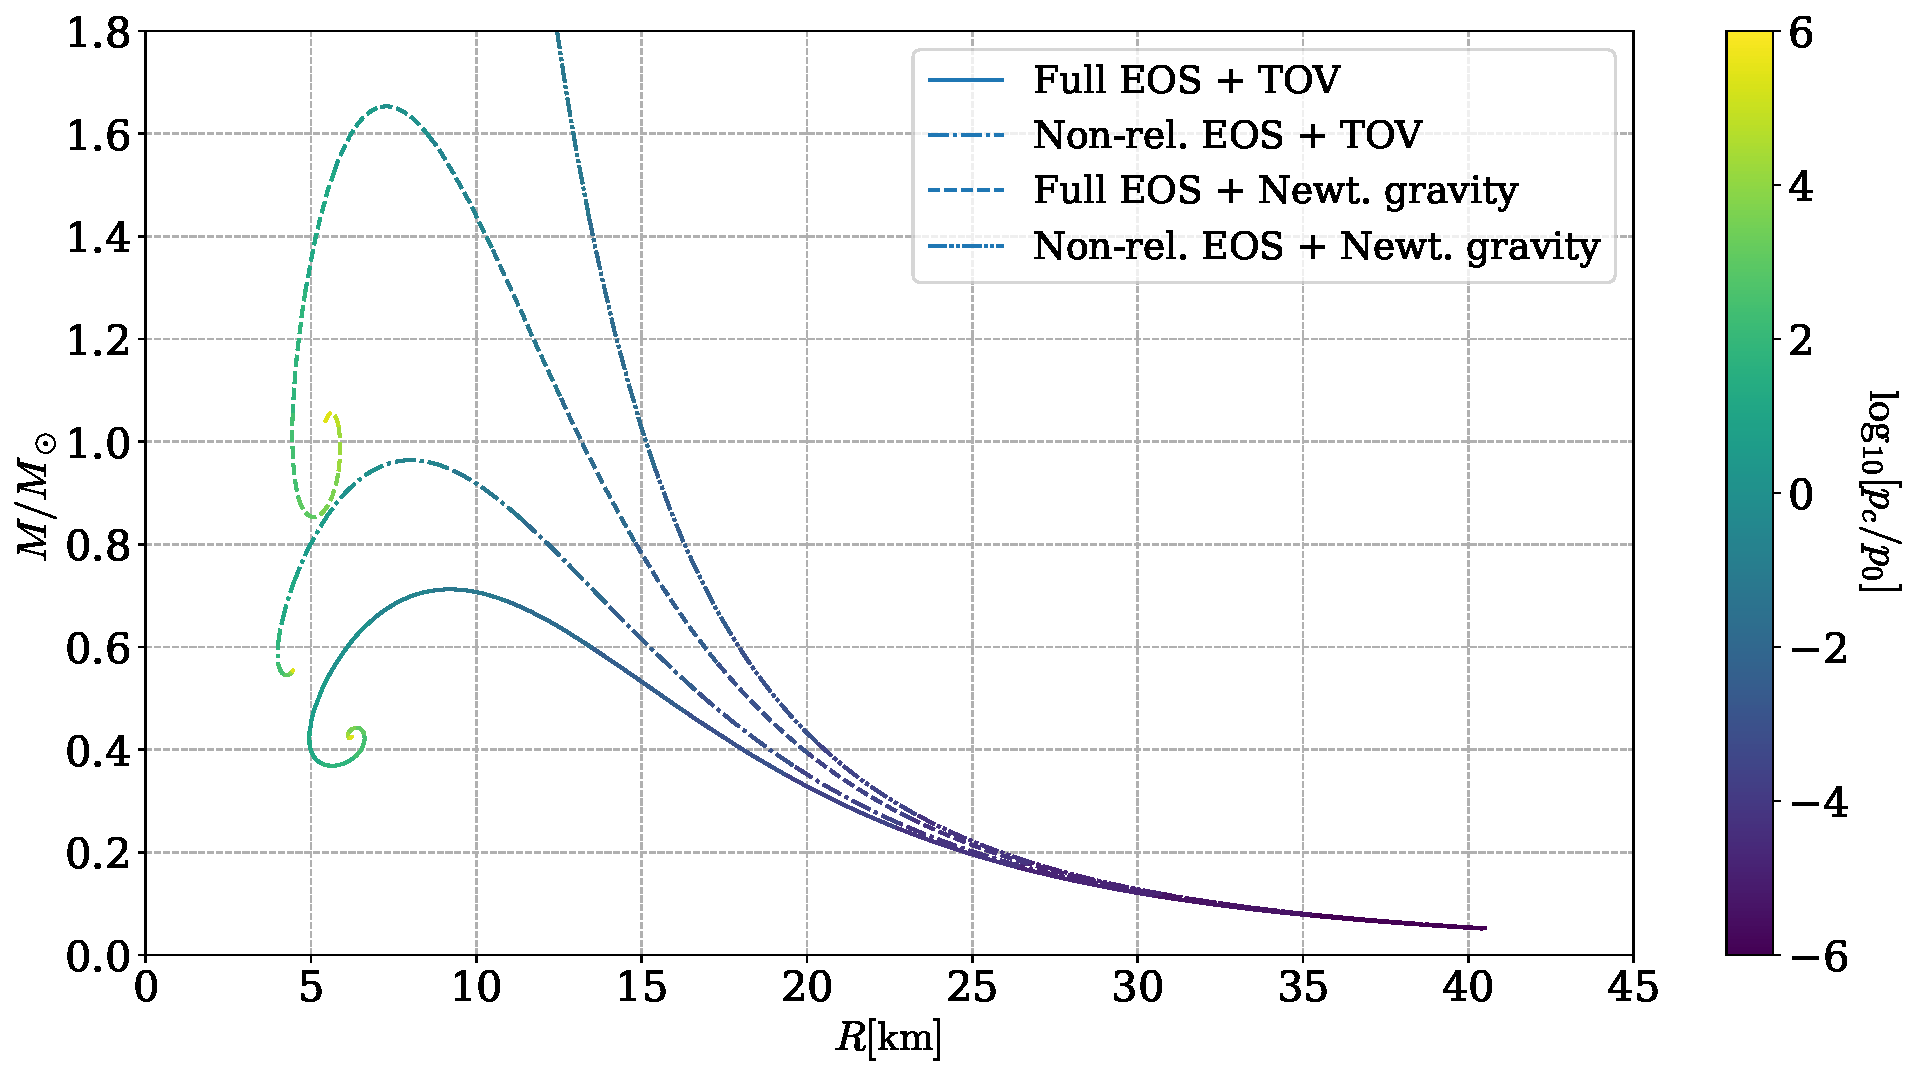
\includegraphics[width=\textwidth]{../../scripts/figurer/mass_radius_comparison.pdf}
        \end{textblock}

        \begin{itemize}
            \item Newtonian limit for TOV,\\
            $\odv{P}{r} = -\frac{G m u}{r^2}$\\
            plus polytrope, $P = K u^\gamma$,  \\
            $\implies \xi^{-2} \odv{}{\xi}\xi^2 \odv{\theta}{\xi} = -\theta^{1/(\gamma - 1)} $,\\
            where $\xi \propto r, \, \theta \propto P^{1/(1-\gamma)}$
            \item Used to derive Chandrasekhar limit
            \item Non-relativistic limit of pion equation of state is polytrope, $P = Ku^2$
            \item We can show that radius is independent of external pressure, and $R = \frac{\pi r^0}{\sqrt{12}}$.
        \end{itemize}

    \end{frame}


    \begin{frame}
        \frametitle{Polytrope mass-radius relation}
        $$M = R^{\beta}$$
        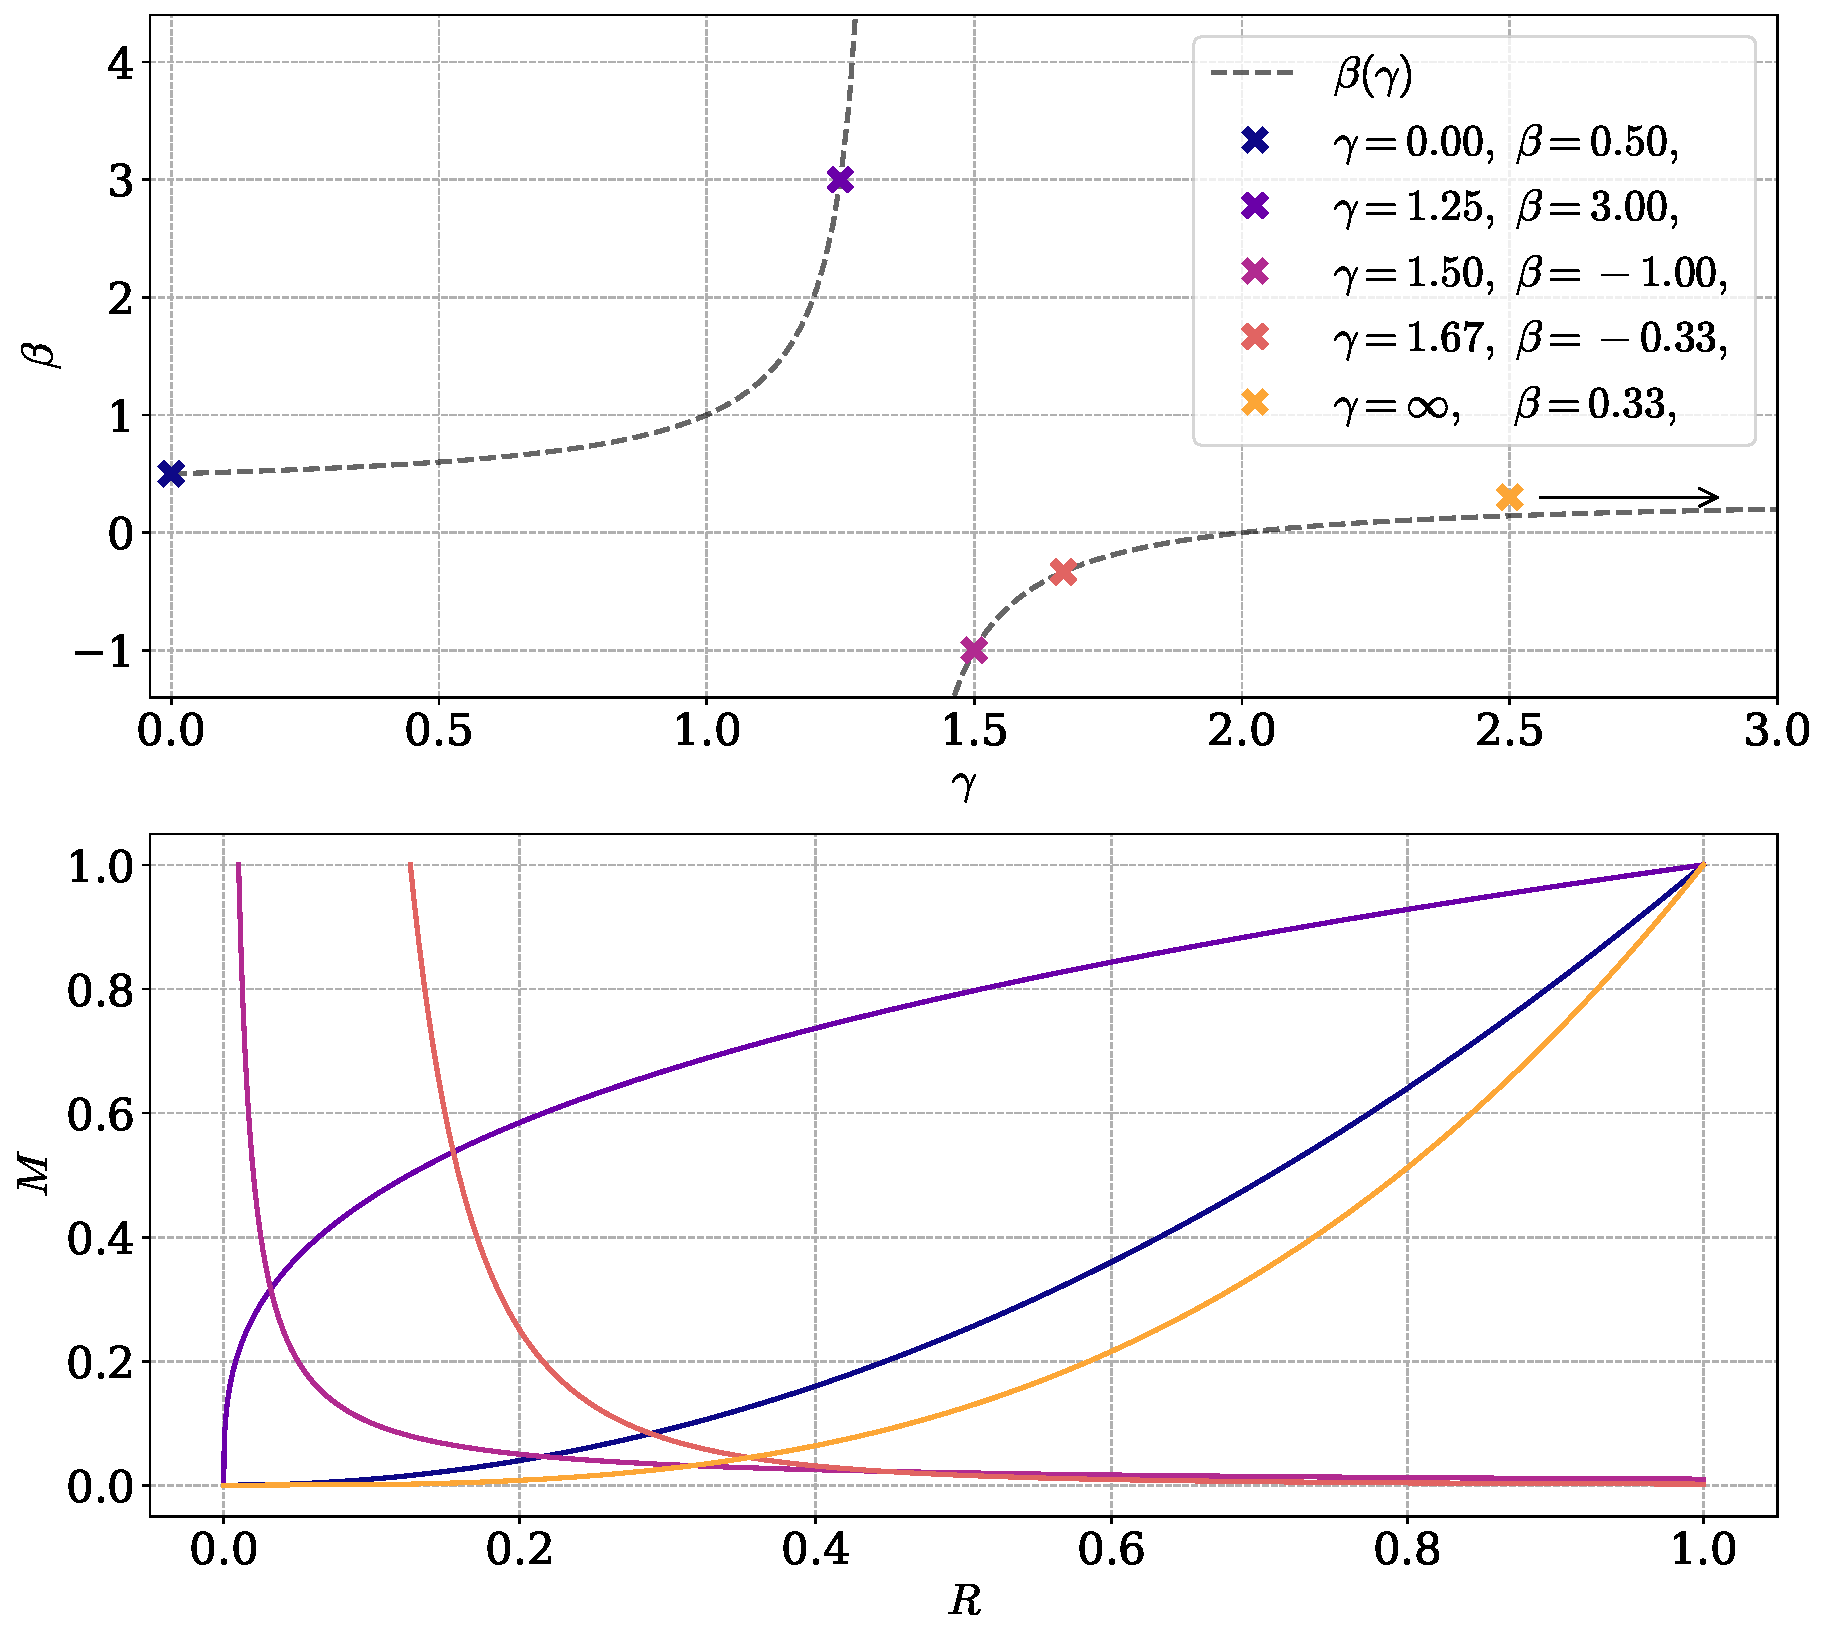
\includegraphics[width=\textwidth]{../../scripts/figurer/mass_radius_relation_polytropes.pdf}
    \end{frame}

    \begin{frame}
        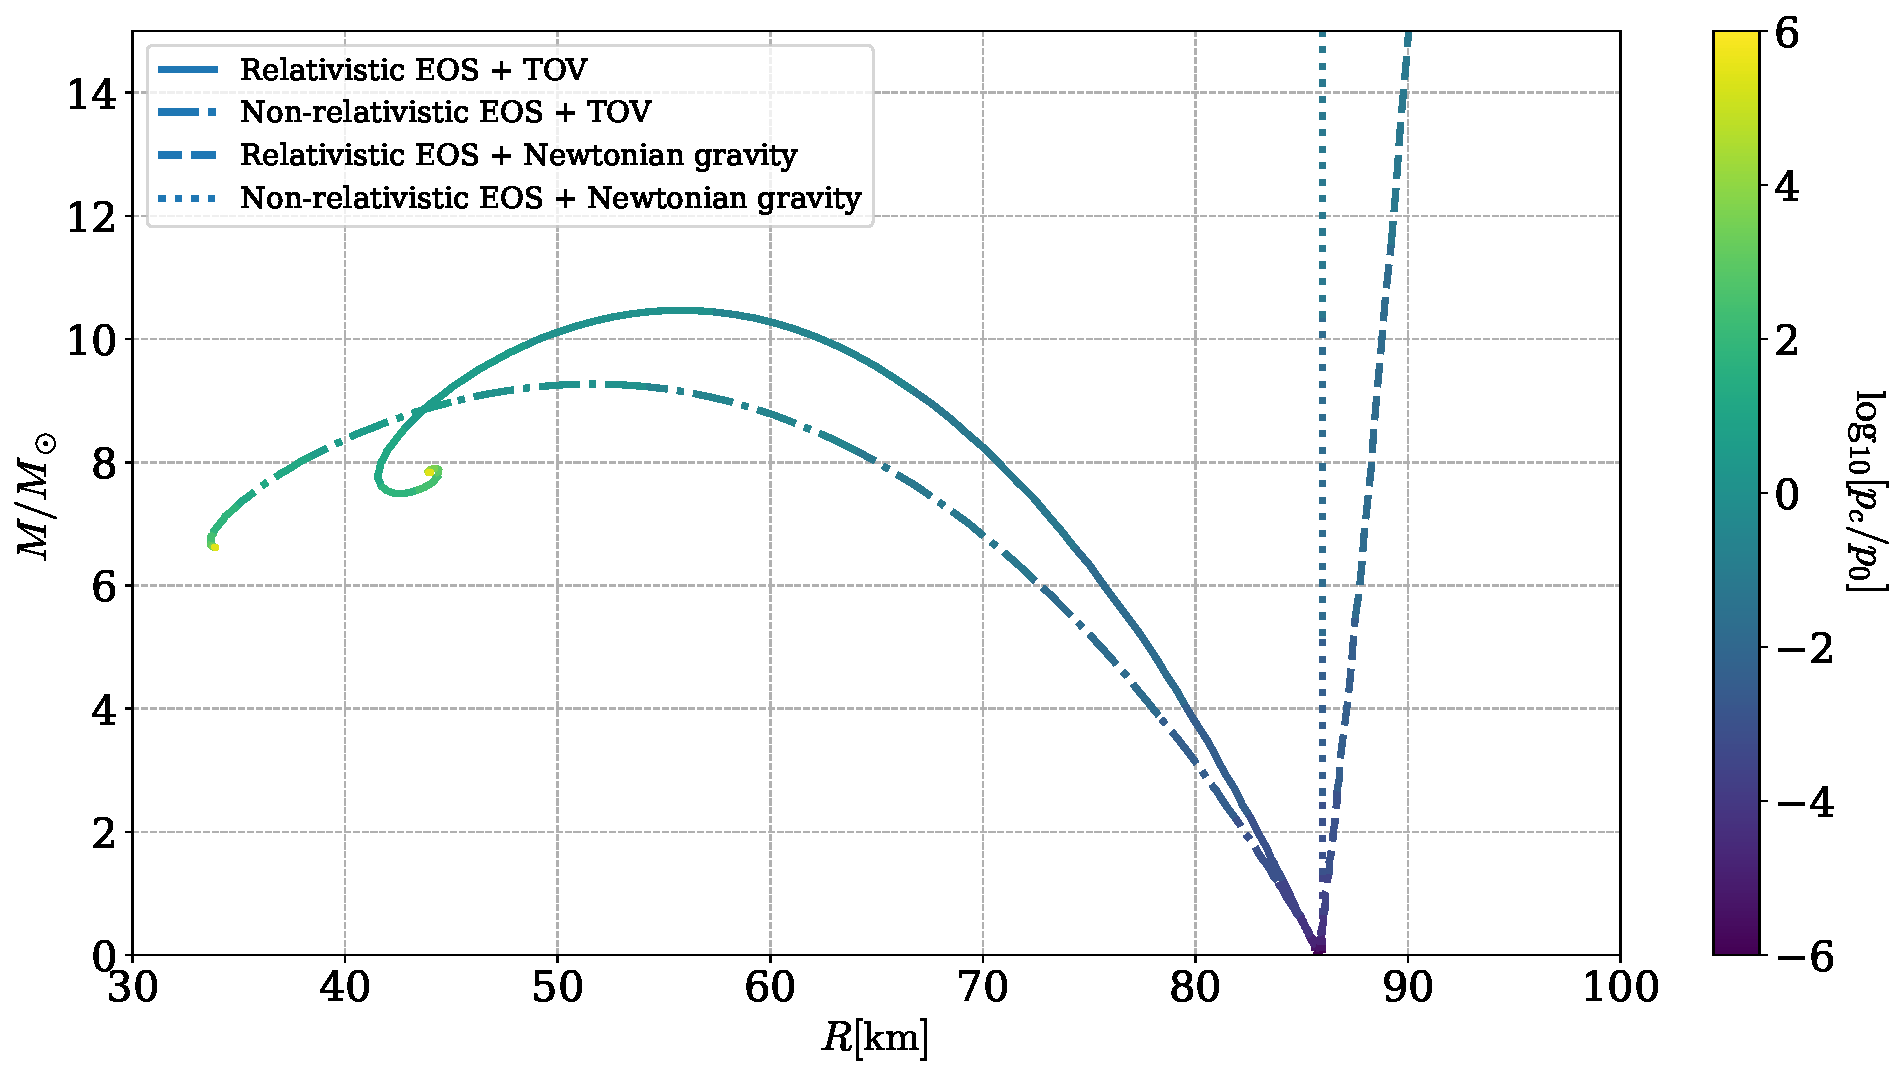
\includegraphics[width=\textwidth]{../../scripts/figurer/pion_star/mass_radius_comparison.pdf}
    \end{frame}

    \begin{frame}
        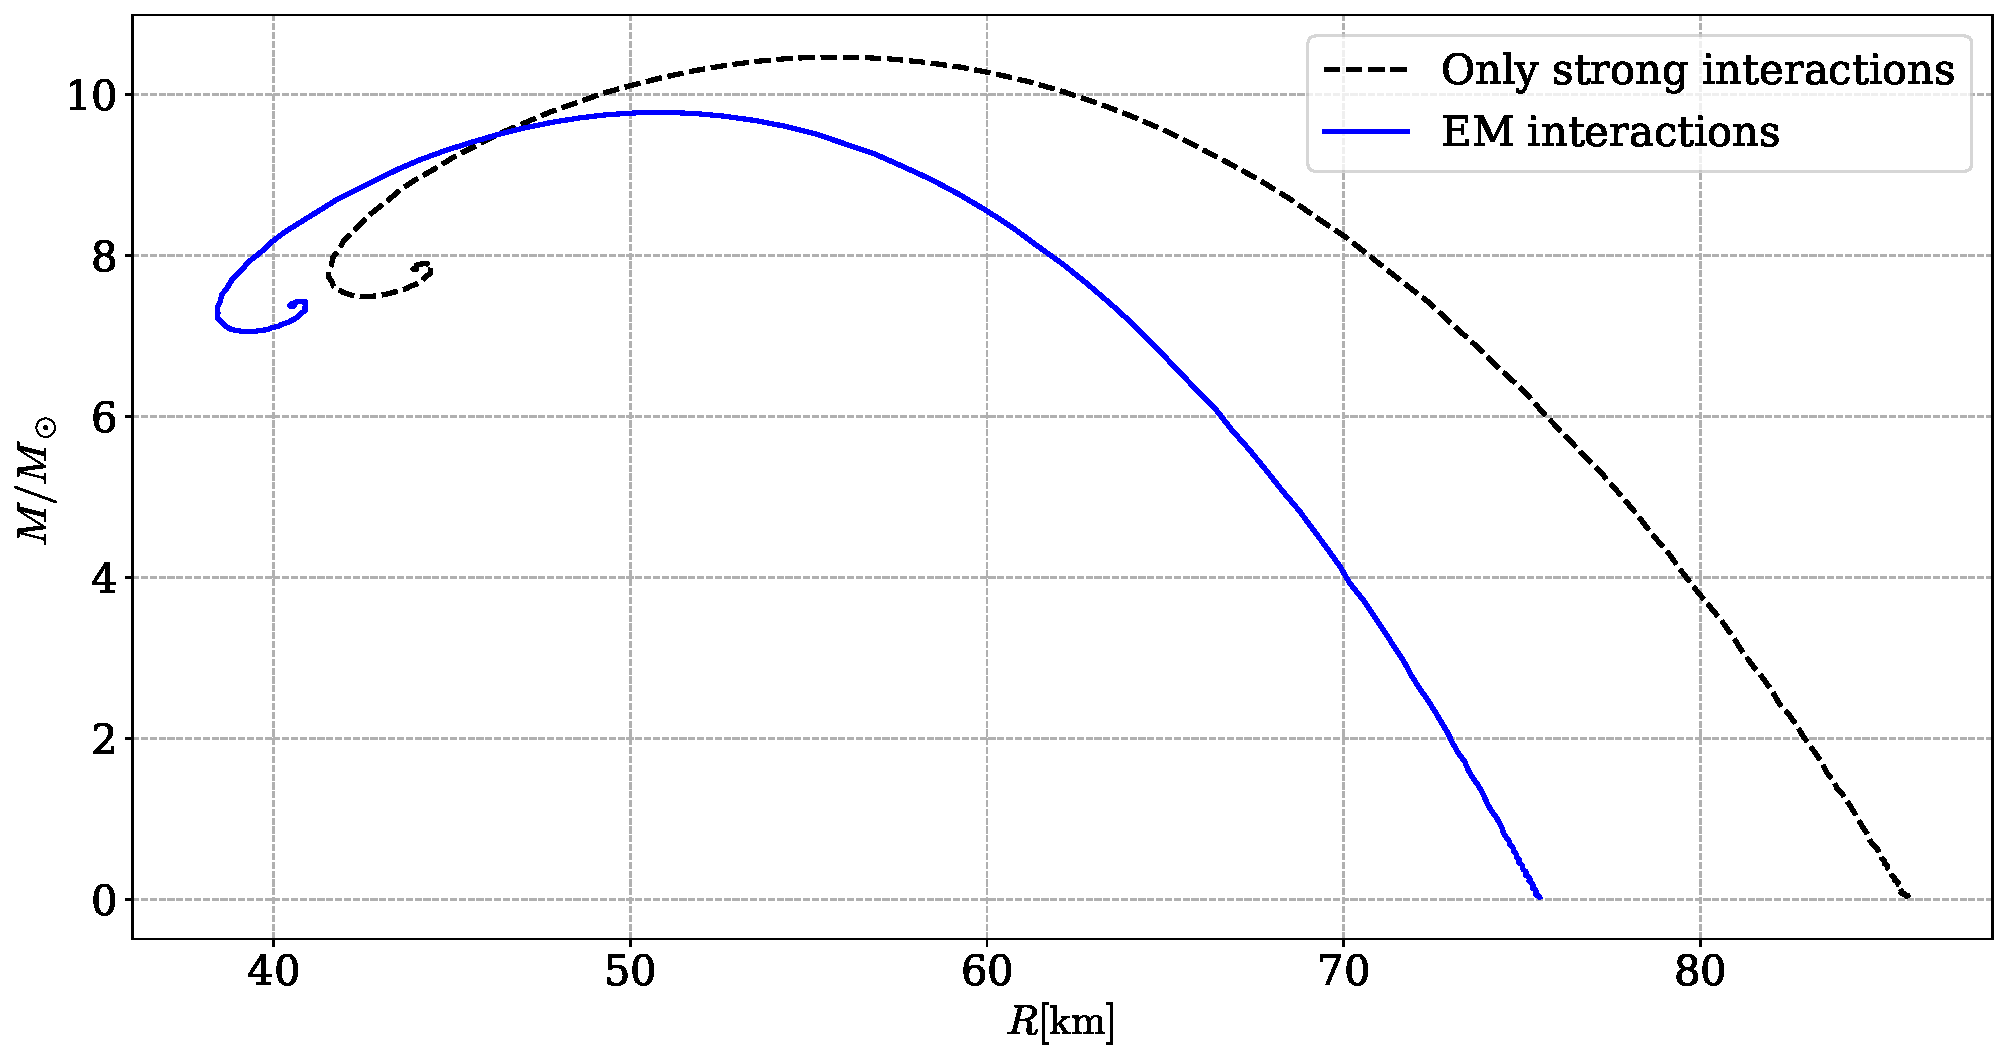
\includegraphics[width=\textwidth]{../../scripts/figurer/pion_star/mass_radius_pion_star_compare.pdf}
    \end{frame}


\end{document}
